% ============================================================
% APPENDIX D -- ADDITIONAL RESULTS (written 2026-11-06)
% Appendix floats referenced from Results (sec:results): per-run trial clouds (figA1, figA2), community
% releases (figA3), per-run search convergence (figA4), and the exact-value tables behind Figures
% fig:kl-budget, fig:capability and fig:divergence (paper/tables/t1--t3, written by
% scripts/make_results_tables.py; do not edit those files by hand). Captions of figA1--A4 are verbatim from
% paper/figures/captions.md (cross-references converted to \ref).
% ============================================================
\section{Additional Results}
\label{app:additional-results}

This appendix gives the per-run optimisation traces and the exact values
behind several main-text figures. Figures~\ref{fig:trials-old}
and~\ref{fig:trials-new} show every completed trial of the seed-1 runs of the
older and newer models (Pareto fronts in Figure~\ref{fig:pareto}).
Figure~\ref{fig:community-releases} gives the capability change and
teacher-forced divergence of the eight community releases (refusal in
Figure~\ref{fig:community}), and Figure~\ref{fig:search-runs} the convergence
curve of every run (summary in Figure~\ref{fig:search-convergence}).
Tables~\ref{tab:dev-refusals-main} and~\ref{tab:dev-refusals-small} list the
dev-set keyword refusals of the trial selected at KL budgets of 0.05, 0.1 and
0.2 (Figure~\ref{fig:kl-budget}); Tables~\ref{tab:capability-main}
and~\ref{tab:capability-small} list the benchmark scores
(Figure~\ref{fig:capability}); and Tables~\ref{tab:teacher-forced-main}
and~\ref{tab:teacher-forced-small} list the teacher-forced log-likelihood of
each original model's answers and its shift under each selected model
(Figure~\ref{fig:divergence}). The four $\gamma$-MPOA models, which
Figures~\ref{fig:capability} and~\ref{fig:divergence} include, are not listed
in these tables; their benchmark changes, dev KL and teacher-forced divergence
are printed in Figure~\ref{fig:gmpoa-heldout}(b). Appendices~\ref{app:trunc256}
and~\ref{app:dev-rescore} report the 256- and 100-token checks of H3 and the
dev-set re-score of the released exports; Appendices~\ref{app:kl-cap},
\ref{app:item-source} and~\ref{app:harm} report the KL-cap binding, the
pair-level pooling and the two scales, the item-source analysis and harmful
compliance as the outcome.
% review revision 2026-11-06: navigation sentence for the new subsections D.3--D.5 (08g, 08h) added.
% src (2026-11-06 fact-check pass): paper/tables/t2_capability_main.tex, t3_teacher_forced_main.tex (no gamma-MPOA rows;
% written by scripts/make_results_tables.py, outside the editable tree); values: results/analysis/final_gmpoa_control.csv,
% final_gmpoa_benchmarks.csv; paper/figures/captions.md (fig12 (b): benchmark deltas, dev KL, teacher-forced divergence)

\begin{figure*}[tp]
\centering
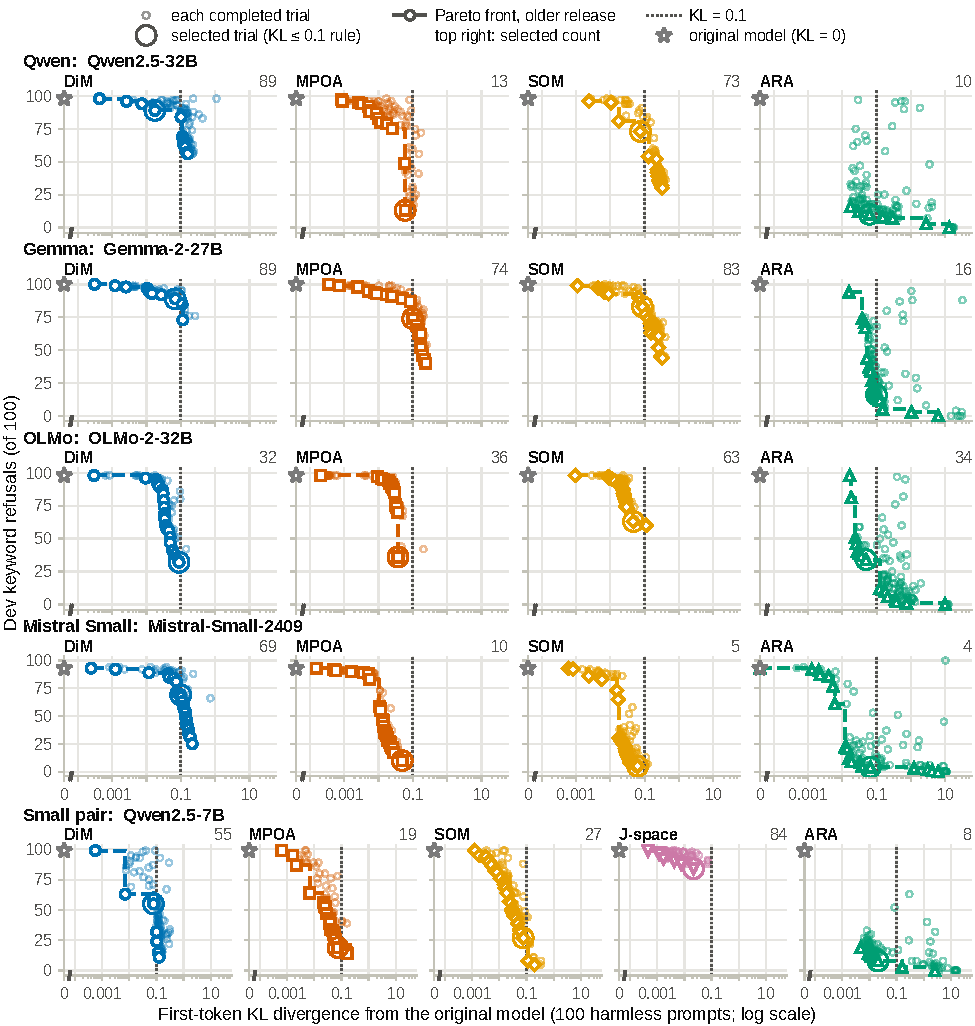
\includegraphics[width=\textwidth]{figures/figA1_trials_old_generation.pdf}
\caption{\textbf{All completed TPE trials of each optimisation run, older releases (dev set).} One panel per run (model $\times$ method, seed 1), laid out as in Figure~\ref{fig:pareto}; the older model of each pair heads its row. Each dot is one completed trial; the line is the run's Pareto front (dashed, hollow markers), the ring the trial chosen by the selection rule (fewest dev keyword refusals at KL $\le$ 0.1; count at the top right of the panel) and the grey star the original model (KL = 0). The x axis is logarithmic, with KL = 0 drawn at the left edge behind an axis break; the dotted line is the selection budget KL = 0.1. 2100 trials from 21 runs; the newer releases are in Figure~\ref{fig:trials-new}. Refusal counts are keyword matches on the 100 dev prompts that were also used for optimisation and selection, not held-out refusal rates.}
\label{fig:trials-old}
\end{figure*}
% caption: paper/figures/captions.md (figA1_trials_old_generation)

\begin{figure*}[tp]
\centering
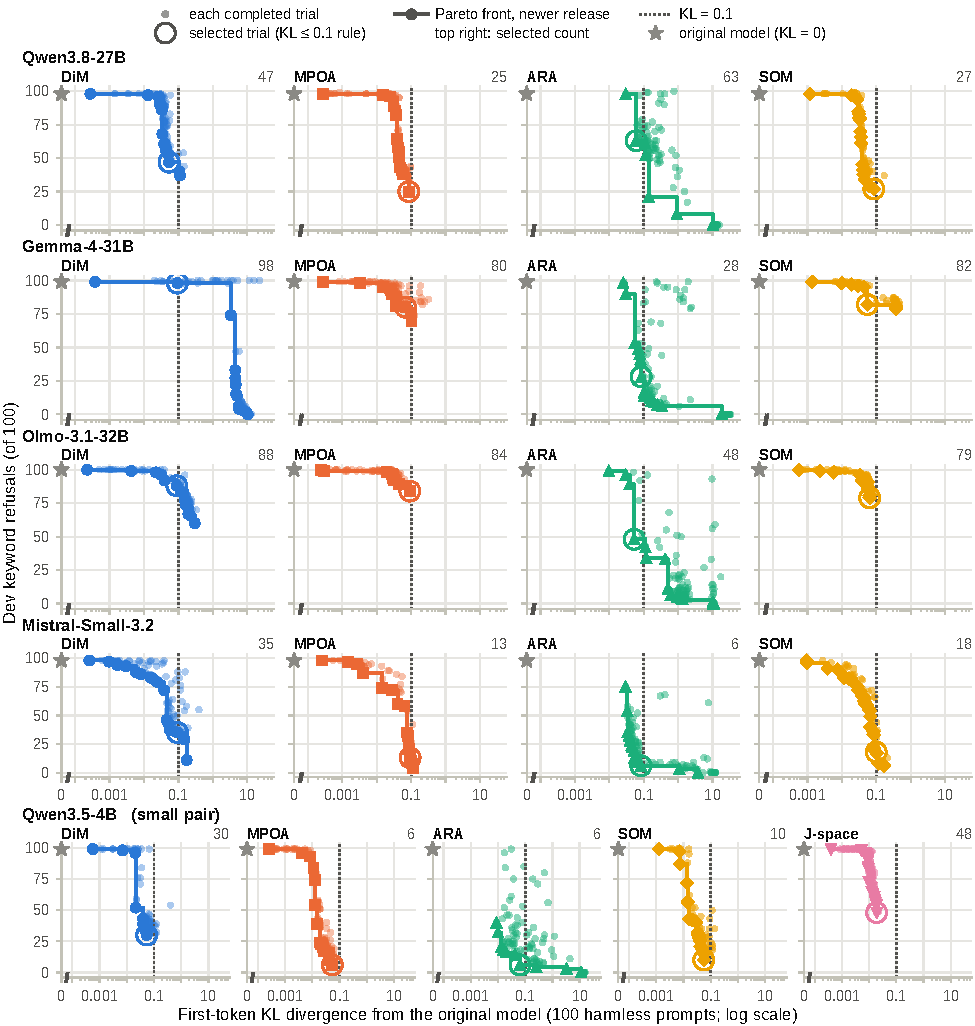
\includegraphics[width=\textwidth]{figures/figA2_trials_new_generation.pdf}
\caption{\textbf{All completed TPE trials of each optimisation run, newer releases (dev set).} One panel per run (model $\times$ method, seed 1), laid out as in Figure~\ref{fig:pareto}; the newer model of each pair heads its row. Each dot is one completed trial; the line is the run's Pareto front (solid, filled markers), the ring the trial chosen by the selection rule (fewest dev keyword refusals at KL $\le$ 0.1; count at the top right of the panel) and the grey star the original model (KL = 0). The x axis is logarithmic, with KL = 0 drawn at the left edge behind an axis break; the dotted line is the selection budget KL = 0.1. 2099 trials from 21 runs; the older releases are in Figure~\ref{fig:trials-old}. Refusal counts are keyword matches on the 100 dev prompts that were also used for optimisation and selection, not held-out refusal rates.}
\label{fig:trials-new}
\end{figure*}
% caption: paper/figures/captions.md (figA2_trials_new_generation)

\begin{figure*}[tp]
\centering
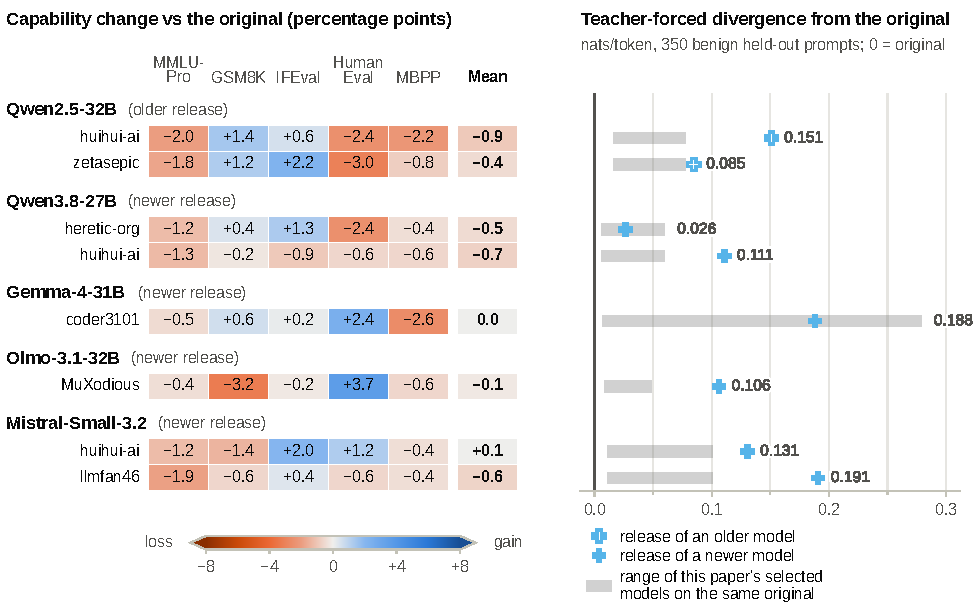
\includegraphics[width=\textwidth]{figures/figA3_community_releases.pdf}
\caption{\textbf{Public community releases: capability change and divergence from the original.} The 8 community releases evaluated alongside the selected models (2 of older, 6 of newer models; row label = Hugging Face uploader), grouped by the original they were derived from. Left: benchmark score minus that of the same original, in percentage points, with the diverging scale of Figure~\ref{fig:capability} (saturating at $\pm$8 pp; printed values exact); the last column is the unweighted mean of the five benchmarks. Right: teacher-forced divergence on the 350 benign held-out prompts, defined as in Figure~\ref{fig:divergence} (0 = the original); hollow markers are releases of the older, filled of the newer model of a pair. The grey bar spans the divergences of this paper's selected models on the same original (all conditions of Figure~\ref{fig:divergence}). 6 of 8 releases lie above that range; divergences range from 0.026 (heretic-org, Qwen3.8-27B) to 0.191 (llmfan46, Mistral-Small-3.2) nats per token, and mean capability changes from $-$0.9 to +0.1 pp. The releases were made by third parties with their own methods and selection; they were not selected with this paper's rule and are not part of the H1--H3 tests.}
\label{fig:community-releases}
\end{figure*}
% caption: paper/figures/captions.md (figA3_community_releases)

\begin{figure*}[tp]
\centering
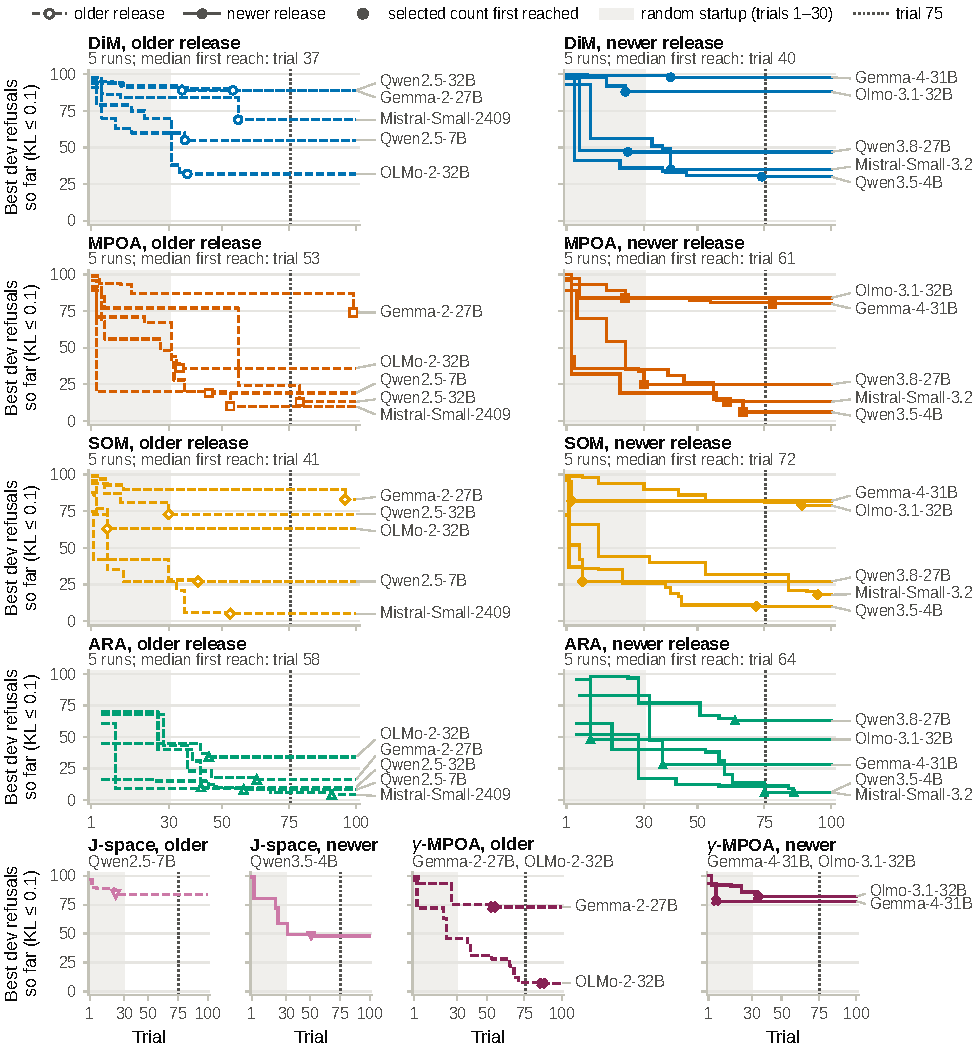
\includegraphics[width=\textwidth]{figures/figA4_search_convergence_runs.pdf}
\caption{\textbf{Search-budget convergence of every optimisation run (dev set).} One step curve per run (seed 1): after trial $t$, the fewest dev keyword refusals (of 100) among trials 1 to $t$ with first-token KL divergence $\le$ 0.1 from the original, i.e. the count the selection rule would have returned had the search stopped at trial $t$. Rows are methods and columns the older and newer release of each pair, so that a panel holds at most five runs, each named at its right end; bottom row: J-space (small pair only) and $\gamma$-MPOA (Gemma and OLMo pairs only). Dashed lines with hollow markers are older, solid lines with filled markers newer releases; the marker sits where the run first reached the count it finally selected. Curves start at the run's first trial within the KL budget (trials 5--10 for ARA, 1--2 otherwise). The grey band marks the 30 random startup trials of the TPE sampler, the dotted line trial 75. The medians, spreads and first-reach histogram of the core runs are in Figure~\ref{fig:search-convergence}. All counts are keyword matches on the 100 dev prompts that were also used for search and selection, not held-out refusal rates.}
\label{fig:search-runs}
\end{figure*}
% caption: paper/figures/captions.md (figA4_search_convergence_runs)

% Auto-generated by scripts/make_results_tables.py at 2026-11-06T06:33:50Z -- do not edit by hand.
\begin{table*}[t]
\centering\small
\caption{Keyword refusals on the development set (mlabonne/harmful\_behaviors, test split, first 100 prompts; count out of 100, Heretic keyword scorer) for the trial selected at each first-token KL budget $\tau$ (KL on mlabonne/harmless\_alpaca, test split, first 100 prompts). Selection rule: among completed trials with KL $\le\tau$, fewest refusals; ties broken by lower KL, then lower trial index. ``Original'' is the unmodified model as recorded by Heretic in the same runs. Main study; seed 1; 100 trials planned per run. $^\dagger$Run with fewer completed than planned trials (Qwen3.8-27B MPOA: 99 of 100). --: not yet available.}
\label{tab:dev-refusals-main}
\begin{tabular}{llrrrrrrrr}
\toprule
 & & \multicolumn{2}{c}{Qwen} & \multicolumn{2}{c}{Gemma} & \multicolumn{2}{c}{OLMo} & \multicolumn{2}{c}{Mistral Small} \\
\cmidrule(lr){3-4}\cmidrule(lr){5-6}\cmidrule(lr){7-8}\cmidrule(lr){9-10}
Method & $\tau$ & 2.5-32B & 3.8-27B & 2-27B & 4-31B & 2-32B & 3.1-32B & 2409 & 3.2-24B \\
\midrule
Original & & 98 & 98 & 100 & 99 & 98 & 100 & 93 & 98 \\
\midrule
DiM & 0.05 & 89 & 53 & 92 & 99 & 47 & 92 & 85 & 46 \\
 & 0.1 & 89 & 47 & 89 & 98 & 32 & 88 & 69 & 35 \\
 & 0.2 & 56 & 37 & 73 & 98 & 32 & 67 & 31 & 11 \\
\midrule
MPOA & 0.05 & 75 & 43$^\dagger$ & 89 & 81 & 36 & 89 & 10 & 60 \\
 & 0.1 & 13 & 25$^\dagger$ & 74 & 80 & 36 & 84 & 10 & 13 \\
 & 0.2 & 13 & 25$^\dagger$ & 46 & 70 & 36 & 84 & 10 & 4 \\
\midrule
ARA & 0.05 & 12 & 98 & 67 & 90 & 34 & 89 & 5 & 22 \\
 & 0.1 & 10 & 63 & 16 & 28 & 34 & 48 & 4 & 6 \\
 & 0.2 & 8 & 21 & 5 & 9 & 10 & 34 & 4 & 6 \\
\midrule
SOM & 0.05 & 81 & 34 & 93 & 95 & 63 & 92 & 8 & 60 \\
 & 0.1 & 73 & 27 & 83 & 82 & 63 & 79 & 5 & 18 \\
 & 0.2 & 54 & 27 & 63 & 82 & 60 & 79 & 5 & 6 \\
\bottomrule
\end{tabular}
\end{table*}
% src: paper/tables/t1_dev_refusals.csv (built from selection.json files; per-cell source_file column)
% src: runs/mc-h200-1/results/bench/mistral-small-2409__ara/selection.json, runs/mc-h200-1/results/bench/mistral-small-2409__dim/selection.json, runs/mc-h200-1/results/bench/mistral-small-2409__mpoa/selection.json, runs/mc-h200-1/results/bench/mistral-small-2409__som/selection.json, runs/mc-h200-1/results/bench/mistral-small-3.2__ara/selection.json, runs/mc-h200-1/results/bench/mistral-small-3.2__dim/selection.json, runs/mc-h200-1/results/bench/mistral-small-3.2__mpoa/selection.json, runs/mc-h200-1/results/bench/mistral-small-3.2__som/selection.json, runs/mc-h200-1/results/bench/olmo-2-32b__ara/selection.json, runs/mc-h200-1/results/bench/olmo-2-32b__dim/selection.json, runs/mc-h200-1/results/bench/olmo-2-32b__mpoa/selection.json, runs/mc-h200-1/results/bench/olmo-2-32b__som/selection.json, runs/mc-h200-1/results/bench/olmo-3.1-32b__ara/selection.json, runs/mc-h200-1/results/bench/olmo-3.1-32b__dim/selection.json, runs/mc-h200-1/results/bench/olmo-3.1-32b__mpoa/selection.json, runs/mc-h200-1/results/bench/olmo-3.1-32b__som/selection.json, runs/mc-rtx-1/results/bench/gemma-2-27b__ara/selection.json, runs/mc-rtx-1/results/bench/gemma-2-27b__dim/selection.json, runs/mc-rtx-1/results/bench/gemma-2-27b__mpoa/selection.json, runs/mc-rtx-1/results/bench/gemma-2-27b__som/selection.json, runs/mc-rtx-1/results/bench/gemma-4-31b__ara/selection.json, runs/mc-rtx-1/results/bench/gemma-4-31b__dim/selection.json, runs/mc-rtx-1/results/bench/gemma-4-31b__mpoa/selection.json, runs/mc-rtx-1/results/bench/gemma-4-31b__som/selection.json, runs/mc-rtx-1/results/bench/qwen2.5-32b__ara/selection.json, runs/mc-rtx-1/results/bench/qwen2.5-32b__dim/selection.json, runs/mc-rtx-1/results/bench/qwen2.5-32b__mpoa/selection.json, runs/mc-rtx-1/results/bench/qwen2.5-32b__som/selection.json, runs/mc-rtx-1/results/bench/qwen3.8-27b__ara/selection.json, runs/mc-rtx-1/results/bench/qwen3.8-27b__dim/selection.json, runs/mc-rtx-1/results/bench/qwen3.8-27b__mpoa/selection.json, runs/mc-rtx-1/results/bench/qwen3.8-27b__som/selection.json
% src: ../heretic/config.default.toml (KeywordRate: mlabonne/harmful_behaviors test[:100]; KLDivergence: mlabonne/harmless_alpaca test[:100]); scripts/select_trial.py (selection rule)
% src: seed, n_trials_planned, n_trials_complete: the selection.json files above (study settings stored in each Optuna journal); configs/core_{dim,mpoa,ara,som,jspace}.toml
% Missing cells rendered as '--' (status from the CSV):
%   none


% Auto-generated by scripts/make_results_tables.py at 2026-11-06T06:33:50Z -- do not edit by hand.
\begin{table}[t]
\centering\small
\caption{Keyword refusals on the development set (mlabonne/harmful\_behaviors, test split, first 100 prompts; count out of 100, Heretic keyword scorer) for the trial selected at each first-token KL budget $\tau$ (KL on mlabonne/harmless\_alpaca, test split, first 100 prompts). Selection rule: among completed trials with KL $\le\tau$, fewest refusals; ties broken by lower KL, then lower trial index. ``Original'' is the unmodified model as recorded by Heretic in the same runs. Small pair; seed 1; 100 trials planned per run. --: not yet available.}
\label{tab:dev-refusals-small}
\begin{tabular}{llrr}
\toprule
 & & \multicolumn{2}{c}{Qwen (small pair)} \\
\cmidrule(lr){3-4}
Method & $\tau$ & 2.5-7B & 3.5-4B \\
\midrule
Original & & 99 & 99 \\
\midrule
DiM & 0.05 & 63 & 34 \\
 & 0.1 & 55 & 30 \\
 & 0.2 & 11 & 30 \\
\midrule
MPOA & 0.05 & 33 & 10 \\
 & 0.1 & 19 & 6 \\
 & 0.2 & 14 & 6 \\
\midrule
ARA & 0.05 & 8 & 14 \\
 & 0.1 & 8 & 6 \\
 & 0.2 & 3 & 6 \\
\midrule
SOM & 0.05 & 39 & 19 \\
 & 0.1 & 27 & 10 \\
 & 0.2 & 5 & 10 \\
\midrule
J-space & 0.05 & 84 & 48 \\
 & 0.1 & 84 & 48 \\
 & 0.2 & 84 & 48 \\
\bottomrule
\end{tabular}
\end{table}
% src: paper/tables/t1_dev_refusals.csv (built from selection.json files; per-cell source_file column)
% src: results/bench-4090/qwen2.5-7b__ara/selection.json, results/bench-4090/qwen2.5-7b__dim/selection.json, results/bench-4090/qwen2.5-7b__jspace/selection.json, results/bench-4090/qwen2.5-7b__mpoa/selection.json, results/bench-4090/qwen2.5-7b__som/selection.json, results/bench-4090/qwen3.5-4b__ara/selection.json, results/bench-4090/qwen3.5-4b__dim/selection.json, results/bench-4090/qwen3.5-4b__jspace/selection.json, results/bench-4090/qwen3.5-4b__mpoa/selection.json, results/bench-4090/qwen3.5-4b__som/selection.json
% src: ../heretic/config.default.toml (KeywordRate: mlabonne/harmful_behaviors test[:100]; KLDivergence: mlabonne/harmless_alpaca test[:100]); scripts/select_trial.py (selection rule)
% src: seed, n_trials_planned, n_trials_complete: the selection.json files above (study settings stored in each Optuna journal); configs/core_{dim,mpoa,ara,som,jspace}.toml
% Missing cells rendered as '--' (status from the CSV):
%   none


% t2_capability_main.tex is 60pt wider than the text at \footnotesize; it is auto-generated (do not edit), so it
% is set here with narrower column gaps and a 7.5pt font, local to this group.
{\setlength{\tabcolsep}{3pt}\renewcommand{\footnotesize}{\fontsize{7.5}{9}\selectfont}%
% Auto-generated by scripts/make_results_tables.py at 2026-11-06T06:33:50Z -- do not edit by hand.
\begin{table*}[t]
\centering\footnotesize
\caption{Capability of the original and the selected modified models (KL $\le 0.1$ trial), in \%. Modified models: score with the difference to the same family's original model in percentage points in parentheses (computed from unrounded scores). Number of items in the column header. Metrics: MMLU-Pro exact match (custom extract, 5-shot CoT); GSM8K exact match (flexible extract, 5-shot); IFEval prompt-level strict accuracy (0-shot); HumanEval pass@1 (0-shot); MBPP pass@1 (3-shot). Greedy decoding, chat template on, thinking disabled. Main study. $^\ddagger$Rescored from the logged samples with the patched MBPP answer extractor (run predates the lm-eval patch; scripts/bench/LM\_EVAL\_PATCHES.md): Qwen2.5-32B-Instruct Original MBPP. $^\S$Original model's capability run used evaluation-harness settings that differ from its modified models' runs (original vs.\ modified models; per-cell settings in paper/tables/coverage.md, evaluation protocol table): Qwen2.5-32B-Instruct: bench.py revision (sha256 prefix) 0ac2aca202 vs.\ b6a926cf73, f220db7bb9; output post-processing none vs.\ U+2581$\rightarrow$space; BENCH\_VLLM\_EXTRA unset vs.\ \{\}. gemma-2-27b-it: bench.py revision (sha256 prefix) b6a926cf73 vs.\ f220db7bb9. --: not yet available.}
\label{tab:capability-main}
\begin{tabular}{llrrrrr}
\toprule
Model & Method & MMLU-Pro (1000) & GSM8K (500) & IFEval (541) & HumanEval (164) & MBPP (500) \\
\midrule
Qwen2.5-32B-Instruct & Original$^\S$ & 71.1 & 85.4 & 78.9 & 89.6 & 77.6$^\ddagger$ \\
 & DiM & 69.9\,($-$1.2) & 85.6\,(+0.2) & 79.7\,(+0.7) & 90.2\,(+0.6) & 77.0\,($-$0.6) \\
 & MPOA & 70.5\,($-$0.6) & 85.0\,($-$0.4) & 80.8\,(+1.8) & 89.6\,(0.0) & 76.6\,($-$1.0) \\
 & ARA & 70.3\,($-$0.8) & 86.6\,(+1.2) & 79.9\,(+0.9) & 84.8\,($-$4.9) & 77.0\,($-$0.6) \\
 & SOM & 71.1\,(0.0) & 85.6\,(+0.2) & 79.5\,(+0.6) & 89.6\,(0.0) & 78.4\,(+0.8) \\
\midrule
Qwen3.8-27B & Original & 79.6 & 96.2 & 80.6 & 97.6 & 80.8 \\
 & DiM & 79.5\,($-$0.1) & 96.6\,(+0.4) & 80.6\,(0.0) & 96.3\,($-$1.2) & 80.6\,($-$0.2) \\
 & MPOA & 79.6\,(0.0) & 97.0\,(+0.8) & 82.4\,(+1.8) & 97.0\,($-$0.6) & 80.4\,($-$0.4) \\
 & ARA & 78.5\,($-$1.1) & 95.8\,($-$0.4) & 81.0\,(+0.4) & 93.9\,($-$3.7) & 79.2\,($-$1.6) \\
 & SOM & 79.4\,($-$0.2) & 97.0\,(+0.8) & 79.5\,($-$1.1) & 95.1\,($-$2.4) & 80.6\,($-$0.2) \\
\midrule
gemma-2-27b-it & Original$^\S$ & 42.8 & 86.4 & 60.6 & 76.2 & 69.6 \\
 & DiM & 42.3\,($-$0.5) & 86.0\,($-$0.4) & 60.6\,(0.0) & 75.0\,($-$1.2) & 69.2\,($-$0.4) \\
 & MPOA & 43.1\,(+0.3) & 84.4\,($-$2.0) & 60.8\,(+0.2) & 76.8\,(+0.6) & 68.6\,($-$1.0) \\
 & ARA & 44.3\,(+1.5) & 84.2\,($-$2.2) & 61.4\,(+0.7) & 76.8\,(+0.6) & 70.0\,(+0.4) \\
 & SOM & 45.3\,(+2.5) & 86.2\,($-$0.2) & 60.8\,(+0.2) & 75.6\,($-$0.6) & 68.6\,($-$1.0) \\
\midrule
gemma-4-31B-it & Original & 85.6 & 96.6 & 91.5 & 92.7 & 71.4 \\
 & DiM & 85.2\,($-$0.4) & 97.0\,(+0.4) & 90.0\,($-$1.5) & 90.2\,($-$2.4) & 69.2\,($-$2.2) \\
 & MPOA & 86.1\,(+0.5) & 96.4\,($-$0.2) & 91.7\,(+0.2) & 90.9\,($-$1.8) & 70.0\,($-$1.4) \\
 & ARA & 85.2\,($-$0.4) & 97.0\,(+0.4) & 91.5\,(0.0) & 86.0\,($-$6.7) & 67.2\,($-$4.2) \\
 & SOM & 85.4\,($-$0.2) & 96.8\,(+0.2) & 89.6\,($-$1.8) & 89.0\,($-$3.7) & 63.0\,($-$8.4) \\
\midrule
OLMo-2-0325-32B-Instruct & Original & 52.6 & 88.8 & 84.3 & 61.0 & 44.0 \\
 & DiM & 52.2\,($-$0.4) & 88.6\,($-$0.2) & 80.8\,($-$3.5) & 59.8\,($-$1.2) & 38.4\,($-$5.6) \\
 & MPOA & 52.3\,($-$0.3) & 88.0\,($-$0.8) & 83.0\,($-$1.3) & 57.9\,($-$3.0) & 42.2\,($-$1.8) \\
 & ARA & 52.3\,($-$0.3) & 88.6\,($-$0.2) & 80.6\,($-$3.7) & 57.3\,($-$3.7) & 30.8\,($-$13.2) \\
 & SOM & 51.9\,($-$0.7) & 88.2\,($-$0.6) & 83.2\,($-$1.1) & 57.9\,($-$3.0) & 44.0\,(0.0) \\
\midrule
Olmo-3.1-32B-Instruct & Original & 64.7 & 89.2 & 86.9 & 87.2 & 71.4 \\
 & DiM & 64.6\,($-$0.1) & 90.4\,(+1.2) & 87.2\,(+0.4) & 88.4\,(+1.2) & 70.2\,($-$1.2) \\
 & MPOA & 63.5\,($-$1.2) & 89.8\,(+0.6) & 86.7\,($-$0.2) & 90.2\,(+3.0) & 71.4\,(0.0) \\
 & ARA & 63.5\,($-$1.2) & 88.6\,($-$0.6) & 87.2\,(+0.4) & 92.1\,(+4.9) & 70.0\,($-$1.4) \\
 & SOM & 64.1\,($-$0.6) & 89.2\,(0.0) & 86.7\,($-$0.2) & 91.5\,(+4.3) & 70.8\,($-$0.6) \\
\midrule
Mistral-Small-Instruct-2409 & Original & 56.2 & 88.2 & 61.4 & 76.2 & 62.6 \\
 & DiM & 56.6\,(+0.4) & 87.4\,($-$0.8) & 62.3\,(+0.9) & 75.6\,($-$0.6) & 61.6\,($-$1.0) \\
 & MPOA & 53.9\,($-$2.3) & 88.0\,($-$0.2) & 61.0\,($-$0.4) & 75.0\,($-$1.2) & 62.2\,($-$0.4) \\
 & ARA & 51.5\,($-$4.7) & 84.2\,($-$4.0) & 63.6\,(+2.2) & 74.4\,($-$1.8) & 58.0\,($-$4.6) \\
 & SOM & 55.6\,($-$0.6) & 88.0\,($-$0.2) & 63.2\,(+1.8) & 76.8\,(+0.6) & 62.4\,($-$0.2) \\
\midrule
Mistral-Small-3.2-24B-Instruct-2506 & Original & 64.8 & 93.6 & 77.1 & 87.2 & 70.6 \\
 & DiM & 64.8\,(0.0) & 93.8\,(+0.2) & 76.9\,($-$0.2) & 87.8\,(+0.6) & 71.2\,(+0.6) \\
 & MPOA & 64.9\,(+0.1) & 94.0\,(+0.4) & 76.0\,($-$1.1) & 89.6\,(+2.4) & 69.6\,($-$1.0) \\
 & ARA & 63.4\,($-$1.4) & 92.6\,($-$1.0) & 77.4\,(+0.4) & 88.4\,(+1.2) & 70.2\,($-$0.4) \\
 & SOM & 63.7\,($-$1.1) & 93.6\,(0.0) & 76.0\,($-$1.1) & 88.4\,(+1.2) & 69.6\,($-$1.0) \\
\bottomrule
\end{tabular}
\end{table*}
% src: paper/tables/t2_capability.csv (built from summary.json 'benchmarks'; per-cell source_file column)
% src: runs/mc-h200-1/results/bench/mistral-small-2409__ara/summary.json, runs/mc-h200-1/results/bench/mistral-small-2409__base/summary.json, runs/mc-h200-1/results/bench/mistral-small-2409__dim/summary.json, runs/mc-h200-1/results/bench/mistral-small-2409__mpoa/summary.json, runs/mc-h200-1/results/bench/mistral-small-2409__som/summary.json, runs/mc-h200-1/results/bench/mistral-small-3.2__ara/summary.json, runs/mc-h200-1/results/bench/mistral-small-3.2__base/summary.json, runs/mc-h200-1/results/bench/mistral-small-3.2__dim/summary.json, runs/mc-h200-1/results/bench/mistral-small-3.2__mpoa/summary.json, runs/mc-h200-1/results/bench/mistral-small-3.2__som/summary.json, runs/mc-h200-1/results/bench/olmo-2-32b__ara/summary.json, runs/mc-h200-1/results/bench/olmo-2-32b__base/summary.json, runs/mc-h200-1/results/bench/olmo-2-32b__dim/summary.json, runs/mc-h200-1/results/bench/olmo-2-32b__mpoa/summary.json, runs/mc-h200-1/results/bench/olmo-2-32b__som/summary.json, runs/mc-h200-1/results/bench/olmo-3.1-32b__ara/summary.json, runs/mc-h200-1/results/bench/olmo-3.1-32b__base/summary.json, runs/mc-h200-1/results/bench/olmo-3.1-32b__dim/summary.json, runs/mc-h200-1/results/bench/olmo-3.1-32b__mpoa/summary.json, runs/mc-h200-1/results/bench/olmo-3.1-32b__som/summary.json, runs/mc-rtx-1/results/bench/gemma-2-27b__ara/summary.json, runs/mc-rtx-1/results/bench/gemma-2-27b__base/summary.json, runs/mc-rtx-1/results/bench/gemma-2-27b__dim/summary.json, runs/mc-rtx-1/results/bench/gemma-2-27b__mpoa/summary.json, runs/mc-rtx-1/results/bench/gemma-2-27b__som/summary.json, runs/mc-rtx-1/results/bench/gemma-4-31b__ara/summary.json, runs/mc-rtx-1/results/bench/gemma-4-31b__base/summary.json, runs/mc-rtx-1/results/bench/gemma-4-31b__dim/summary.json, runs/mc-rtx-1/results/bench/gemma-4-31b__mpoa/summary.json, runs/mc-rtx-1/results/bench/gemma-4-31b__som/summary.json, runs/mc-rtx-1/results/bench/qwen2.5-32b__ara/summary.json, runs/mc-rtx-1/results/bench/qwen2.5-32b__base/summary.json, runs/mc-rtx-1/results/bench/qwen2.5-32b__dim/summary.json, runs/mc-rtx-1/results/bench/qwen2.5-32b__mpoa/summary.json, runs/mc-rtx-1/results/bench/qwen2.5-32b__som/summary.json, runs/mc-rtx-1/results/bench/qwen3.8-27b__ara/summary.json, runs/mc-rtx-1/results/bench/qwen3.8-27b__base/summary.json, runs/mc-rtx-1/results/bench/qwen3.8-27b__dim/summary.json, runs/mc-rtx-1/results/bench/qwen3.8-27b__mpoa/summary.json, runs/mc-rtx-1/results/bench/qwen3.8-27b__som/summary.json
% src: scripts/bench/README.md (protocol: metrics, shots, decoding, chat template, thinking off); metric names and n: summary.json 'benchmarks' (metric, n)
% src (section-sign footnote): summary.json versions['sha256:bench.py'], postprocess, versions.env, backend, lm_kwargs, versions of runs/mc-rtx-1/results/bench/qwen2.5-32b__base/summary.json, runs/mc-rtx-1/results/bench/gemma-2-27b__base/summary.json vs. the modified models' summary.json; paper/tables/coverage.md (evaluation protocol table)
% Missing cells rendered as '--' (status from the CSV):
%   none

}

% Auto-generated by scripts/make_results_tables.py at 2026-11-06T06:33:50Z -- do not edit by hand.
\begin{table*}[t]
\centering\small
\caption{Capability of the original and the selected modified models (KL $\le 0.1$ trial), in \%. Modified models: score with the difference to the same family's original model in percentage points in parentheses (computed from unrounded scores). Number of items in the column header. Metrics: MMLU-Pro exact match (custom extract, 5-shot CoT); GSM8K exact match (flexible extract, 5-shot); IFEval prompt-level strict accuracy (0-shot); HumanEval pass@1 (0-shot); MBPP pass@1 (3-shot). Greedy decoding, chat template on, thinking disabled. Small pair. --: not yet available.}
\label{tab:capability-small}
\setlength{\tabcolsep}{4pt}
\begin{tabular}{llrrrrr}
\toprule
Model & Method & MMLU-Pro (1000) & GSM8K (500) & IFEval (541) & HumanEval (164) & MBPP (500) \\
\midrule
Qwen2.5-7B-Instruct & Original & 59.5 & 85.8 & 71.2 & 84.8 & 63.2 \\
 & DiM & 58.1\,($-$1.4) & 86.0\,(+0.2) & 71.7\,(+0.6) & 86.0\,(+1.2) & 63.8\,(+0.6) \\
 & MPOA & 57.9\,($-$1.6) & 85.0\,($-$0.8) & 70.6\,($-$0.6) & 86.6\,(+1.8) & 63.2\,(0.0) \\
 & ARA & 57.8\,($-$1.7) & 86.8\,(+1.0) & 70.2\,($-$0.9) & 87.2\,(+2.4) & 64.8\,(+1.6) \\
 & SOM & 59.8\,(+0.3) & 84.0\,($-$1.8) & 70.6\,($-$0.6) & 83.5\,($-$1.2) & 64.8\,(+1.6) \\
 & J-space & 60.5\,(+1.0) & 86.4\,(+0.6) & 72.6\,(+1.5) & 84.8\,(0.0) & 64.4\,(+1.2) \\
\midrule
Qwen3.5-4B & Original & 70.6 & 91.8 & 82.3 & 79.9 & 62.6 \\
 & DiM & 70.1\,($-$0.5) & 91.2\,($-$0.6) & 82.4\,(+0.2) & 81.7\,(+1.8) & 61.8\,($-$0.8) \\
 & MPOA & 69.2\,($-$1.4) & 91.6\,($-$0.2) & 82.3\,(0.0) & 79.9\,(0.0) & 61.6\,($-$1.0) \\
 & ARA & 69.4\,($-$1.2) & 90.2\,($-$1.6) & 79.3\,($-$3.0) & 79.3\,($-$0.6) & 61.2\,($-$1.4) \\
 & SOM & 68.7\,($-$1.9) & 92.6\,(+0.8) & 81.7\,($-$0.6) & 79.9\,(0.0) & 61.2\,($-$1.4) \\
 & J-space & 70.4\,($-$0.2) & 91.6\,($-$0.2) & 81.3\,($-$0.9) & 82.9\,(+3.0) & 61.2\,($-$1.4) \\
\bottomrule
\end{tabular}
\end{table*}
% src: paper/tables/t2_capability.csv (built from summary.json 'benchmarks'; per-cell source_file column)
% src: results/bench-4090/qwen2.5-7b__ara/summary.json, results/bench-4090/qwen2.5-7b__base/summary.json, results/bench-4090/qwen2.5-7b__dim/summary.json, results/bench-4090/qwen2.5-7b__jspace/summary.json, results/bench-4090/qwen2.5-7b__mpoa/summary.json, results/bench-4090/qwen2.5-7b__som/summary.json, results/bench-4090/qwen3.5-4b__ara/summary.json, results/bench-4090/qwen3.5-4b__base/summary.json, results/bench-4090/qwen3.5-4b__dim/summary.json, results/bench-4090/qwen3.5-4b__jspace/summary.json, results/bench-4090/qwen3.5-4b__mpoa/summary.json, results/bench-4090/qwen3.5-4b__som/summary.json
% src: scripts/bench/README.md (protocol: metrics, shots, decoding, chat template, thinking off); metric names and n: summary.json 'benchmarks' (metric, n)
% Missing cells rendered as '--' (status from the CSV):
%   none


% Auto-generated by scripts/make_results_tables.py at 2026-11-06T06:33:50Z -- do not edit by hand.
\begin{table*}[t]
\centering\small
\caption{Teacher-forced log-likelihood of the original model's greedy answers to the 350 benign held-out prompts (jbb\_benign 100, xstest\_safe 250). ``Original'': mean log-probability per answer token under the original model (token-weighted over all items); method columns: the same quantity under the selected modified model (KL $\le 0.1$ trial) minus the original's value (negative = the original answers became less likely). Tokens: number of scored answer tokens. Main study. $^\S$Original model's held-out generation and teacher forcing come from a run whose evaluation-harness settings differ from its modified models' runs (original vs.\ modified models; per-cell settings in paper/tables/coverage.md, evaluation protocol table): Qwen2.5-32B-Instruct: separate bench.py run (refusal\_run/summary.json in its evaluation directory); bench.py revision (sha256 prefix) f7731f7d3f vs.\ b6a926cf73, f220db7bb9; output post-processing none vs.\ U+2581$\rightarrow$space. gemma-2-27b-it: bench.py revision (sha256 prefix) b6a926cf73 vs.\ f220db7bb9. --: not yet available.}
\label{tab:teacher-forced-main}
\begin{tabular}{lrrrrrr}
\toprule
 & & & \multicolumn{4}{c}{Shift vs.\ original} \\
\cmidrule(lr){4-7}
Model & Tokens & Original & DiM & MPOA & ARA & SOM \\
\midrule
Qwen2.5-32B-Instruct & 112398 & $-$0.272$^\S$ & $-$0.017 & $-$0.042 & $-$0.077 & $-$0.020 \\
Qwen3.8-27B & 138016 & $-$0.275 & $-$0.006 & $-$0.060 & $-$0.042 & $-$0.021 \\
gemma-2-27b-it & 97666 & $-$0.227$^\S$ & $-$0.068 & $-$0.063 & $-$0.161 & $-$0.031 \\
gemma-4-31B-it & 142322 & $-$0.110 & $-$0.042 & $-$0.007 & $-$0.279 & $-$0.026 \\
OLMo-2-0325-32B-Instruct & 110792 & $-$0.520 & $-$0.051 & $-$0.088 & $-$0.055 & $-$0.030 \\
Olmo-3.1-32B-Instruct & 136772 & $-$0.288 & $-$0.008 & $-$0.008 & $-$0.049 & $-$0.016 \\
Mistral-Small-Instruct-2409 & 129960 & $-$0.209 & $-$0.004 & $-$0.018 & $-$0.080 & $-$0.023 \\
Mistral-Small-3.2-24B-Instruct-2506 & 131780 & $-$0.171 & $-$0.011 & $-$0.066 & $-$0.101 & $-$0.037 \\
\bottomrule
\end{tabular}
\end{table*}
% src: paper/tables/t3_teacher_forced.csv (summary.json 'teacher_forced'; per-cell source_file column)
% src: runs/mc-h200-1/results/bench/mistral-small-2409__ara/summary.json, runs/mc-h200-1/results/bench/mistral-small-2409__base/summary.json, runs/mc-h200-1/results/bench/mistral-small-2409__dim/summary.json, runs/mc-h200-1/results/bench/mistral-small-2409__mpoa/summary.json, runs/mc-h200-1/results/bench/mistral-small-2409__som/summary.json, runs/mc-h200-1/results/bench/mistral-small-3.2__ara/summary.json, runs/mc-h200-1/results/bench/mistral-small-3.2__base/summary.json, runs/mc-h200-1/results/bench/mistral-small-3.2__dim/summary.json, runs/mc-h200-1/results/bench/mistral-small-3.2__mpoa/summary.json, runs/mc-h200-1/results/bench/mistral-small-3.2__som/summary.json, runs/mc-h200-1/results/bench/olmo-2-32b__ara/summary.json, runs/mc-h200-1/results/bench/olmo-2-32b__base/summary.json, runs/mc-h200-1/results/bench/olmo-2-32b__dim/summary.json, runs/mc-h200-1/results/bench/olmo-2-32b__mpoa/summary.json, runs/mc-h200-1/results/bench/olmo-2-32b__som/summary.json, runs/mc-h200-1/results/bench/olmo-3.1-32b__ara/summary.json, runs/mc-h200-1/results/bench/olmo-3.1-32b__base/summary.json, runs/mc-h200-1/results/bench/olmo-3.1-32b__dim/summary.json, runs/mc-h200-1/results/bench/olmo-3.1-32b__mpoa/summary.json, runs/mc-h200-1/results/bench/olmo-3.1-32b__som/summary.json, runs/mc-rtx-1/results/bench/gemma-2-27b__ara/summary.json, runs/mc-rtx-1/results/bench/gemma-2-27b__base/summary.json, runs/mc-rtx-1/results/bench/gemma-2-27b__dim/summary.json, runs/mc-rtx-1/results/bench/gemma-2-27b__mpoa/summary.json, runs/mc-rtx-1/results/bench/gemma-2-27b__som/summary.json, runs/mc-rtx-1/results/bench/gemma-4-31b__ara/summary.json, runs/mc-rtx-1/results/bench/gemma-4-31b__base/summary.json, runs/mc-rtx-1/results/bench/gemma-4-31b__dim/summary.json, runs/mc-rtx-1/results/bench/gemma-4-31b__mpoa/summary.json, runs/mc-rtx-1/results/bench/gemma-4-31b__som/summary.json, runs/mc-rtx-1/results/bench/qwen2.5-32b__ara/summary.json, runs/mc-rtx-1/results/bench/qwen2.5-32b__base/refusal_run/summary.json, runs/mc-rtx-1/results/bench/qwen2.5-32b__dim/summary.json, runs/mc-rtx-1/results/bench/qwen2.5-32b__mpoa/summary.json, runs/mc-rtx-1/results/bench/qwen2.5-32b__som/summary.json, runs/mc-rtx-1/results/bench/qwen3.8-27b__ara/summary.json, runs/mc-rtx-1/results/bench/qwen3.8-27b__base/summary.json, runs/mc-rtx-1/results/bench/qwen3.8-27b__dim/summary.json, runs/mc-rtx-1/results/bench/qwen3.8-27b__mpoa/summary.json, runs/mc-rtx-1/results/bench/qwen3.8-27b__som/summary.json
% src: scripts/bench/bench.py (teacher_forced_logprobs: token-weighted mean over benign items); scripts/bench/refusal_sets.json (benign item counts)
% src (section-sign footnote): settings recorded in runs/mc-rtx-1/results/bench/qwen2.5-32b__base/refusal_run/summary.json, runs/mc-rtx-1/results/bench/gemma-2-27b__base/summary.json vs. the modified models' summary.json; paper/tables/coverage.md (evaluation protocol table)
% Missing cells rendered as '--' (status from the CSV):
%   none


% Auto-generated by scripts/make_results_tables.py at 2026-11-06T06:33:50Z -- do not edit by hand.
\begin{table*}[t]
\centering\small
\caption{Teacher-forced log-likelihood of the original model's greedy answers to the 350 benign held-out prompts (jbb\_benign 100, xstest\_safe 250). ``Original'': mean log-probability per answer token under the original model (token-weighted over all items); method columns: the same quantity under the selected modified model (KL $\le 0.1$ trial) minus the original's value (negative = the original answers became less likely). Tokens: number of scored answer tokens. Small pair. --: not yet available.}
\label{tab:teacher-forced-small}
\begin{tabular}{lrrrrrrr}
\toprule
 & & & \multicolumn{5}{c}{Shift vs.\ original} \\
\cmidrule(lr){4-8}
Model & Tokens & Original & DiM & MPOA & ARA & SOM & J-space \\
\midrule
Qwen2.5-7B-Instruct & 119254 & $-$0.321 & $-$0.019 & $-$0.018 & $-$0.048 & $-$0.026 & $-$0.009 \\
Qwen3.5-4B & 139372 & $-$0.412 & $-$0.010 & $-$0.031 & $-$0.093 & $-$0.035 & $-$0.045 \\
\bottomrule
\end{tabular}
\end{table*}
% src: paper/tables/t3_teacher_forced.csv (summary.json 'teacher_forced'; per-cell source_file column)
% src: results/bench-4090/qwen2.5-7b__ara/summary.json, results/bench-4090/qwen2.5-7b__base/summary.json, results/bench-4090/qwen2.5-7b__dim/summary.json, results/bench-4090/qwen2.5-7b__jspace/summary.json, results/bench-4090/qwen2.5-7b__mpoa/summary.json, results/bench-4090/qwen2.5-7b__som/summary.json, results/bench-4090/qwen3.5-4b__ara/summary.json, results/bench-4090/qwen3.5-4b__base/summary.json, results/bench-4090/qwen3.5-4b__dim/summary.json, results/bench-4090/qwen3.5-4b__jspace/summary.json, results/bench-4090/qwen3.5-4b__mpoa/summary.json, results/bench-4090/qwen3.5-4b__som/summary.json
% src: scripts/bench/bench.py (teacher_forced_logprobs: token-weighted mean over benign items); scripts/bench/refusal_sets.json (benign item counts)
% Missing cells rendered as '--' (status from the CSV):
%   none


% ---------------------------------------------------------------------
% 2026-11-10 ARS re-review revision (NEW-6): diagnosis of the failed Gemma-4-31B DiM edit, replacing the unsupported
% "plausibly for architectural reasons".
% src: scripts/analysis/postnorm_gain_scan.py -> results/analysis/gemma4_dim_kl_bands.csv (from the Optuna journal
% src: runs/mc-h200-1/runs/gemma-4-31b__dim__core-s1/checkpoints/google--gemma-4-31B-it.jsonl) and
% src: results/analysis/postnorm_gain_scan.csv (post-norm weights read from the base-model safetensors on Hugging Face);
% src: results/analysis/review_sel_kl_runs.csv (kl_of_best_above_cap: every other direction-based primary run <= 0.371).
\subsection{The Failed Gemma-4-31B DiM Edit}
\label{app:gemma4-dim}
In the Gemma-4-31B DiM study, 10 of the 100 trials met the KL cap and 90
exceeded it. Every trial with a first-token KL below 3 (28 trials) refused 98
to 100 of the 100 dev prompts; lower refusal appeared only above a KL of 3
(minimum 3 of 100 between 3 and 8, and 0 above 8), where the edited model is
far from the original. In every other direction-based primary study, the
lowest-refusal trial above the cap had a KL of at most 0.37. The edit therefore
did not trade refusal against divergence gradually: within any usable budget it
had no effect. Two mechanisms proposed for similar failures on Gemma-3 are a
residual-stream coordinate of very large magnitude that dominates the
difference-in-means estimate \cite{mishra2026onecoordinate,lai2025mpoa} and
learned normalisation gains that amplify it \cite{mishra2026onecoordinate}. The
post-sublayer RMSNorm gains of the four post-norm models were therefore read
from the released weights. Gemma-2-27B and Gemma-4-31B both had recurring
outlier channels (a gain over 20 times the layer's median in 39 of 92 and 27 of
120 post-norm vectors, mostly one channel in Gemma-2-27B and two in
Gemma-4-31B), whereas OLMo-2-32B and Olmo-3.1-32B had 3 of 128 and 1 of 128.
The median coefficient of variation of the gains was 0.65 and 0.68 for the
attention outputs and 0.38 and 0.62 for the feed-forward outputs of the two
Gemma models, and 0.09 to 0.34 in the OLMo models; outlier channels were more
frequent in Gemma-2-27B than in Gemma-4-31B (42\% and 23\% of vectors). The gains thus separate the Gemma family from
OLMo, consistent with the larger effect of the $\gamma$ correction on the Gemma
models (\S\ref{sec:res-secondary}), but they do not separate Gemma-4-31B from
Gemma-2-27B, on which DiM lowered refusal. The activation outlier was not
measured, and the cause of the failure remains untested.
